%************************************************
\chapter{Methodology}\label{ch:methodology}
%************************************************

The purpose of this chapter is to first formulate the research questions that we examine in our work
and then propose our method of answering them.

\section{Research Questions}\label{sec:research_questions}

In the \nameref{ch:example_chapter} chapter we dicussed the different meanings of structural and dataflow-based interactions.
With this knowledge, we can answer many interesting research topics. 
These topics include patterns in feature development and usage of commits therin as well as findings about how likely seemingly unrelated commits are to affect features inside a program.

\subsection*{\textbf{RQ1: How do commits and features structurally interact with each other?}}

We intend to research two main properties which already provide a lot of insight into the development process of features and best practices of commits therein.

\subsubsection*{Patterns around Feature Development}

Firstly, we examine the number of commits features interact with structurally. 
This gives us a direct estimate on how many commits were used in the development of a feature.
Our analysis also allows us to measure the size of feature, which can put the number of commits used to implement a feature into perspective.
We refine our investigation by factoring in the nesting degrees~\ref{sec:nesting_degree} of our collected structural CFIs.
This allows us to additionally determine the \textsf{definite} size of a feature showing us to what extent its code is nested inside other features.
Furthermore, we can differentiate between commits that most likely and those that only potentially implemented a feature's functionality.
By doing so, we intend to achieve a more accurate analysis regarding the number of commits used during a feature's development.

\subsubsection*{Usage of Commits in Feature Development}

Secondly, we examine how many features a commit interacts with structurally, i.e. how many features a commit usually changes. 
This is especially interesting when considering best practices surrounding the usage of commits.
It is preferred to keep commits atomic\cite{hundhausen2021commit_metrics} meaning they should only deal with a single concern.
As different features implement separate functionalities, it's unlikely for a commit to change several features while dealing with the same concern.
Transferring this to our work, high quality commits should mostly change a single feature.
Acquiring data on this issue might show how strictly this policy is enforced in the development of features across different projects. 
Here, differentiating between the nesting degrees of structural interactions provides us with more informative results. 
We can form a lower bound for the number of features a commit usually changes by only considering structural interactions with a nesting degree of one.
This way we only take into account commits for which we are certain that they were used to specifically implement a feature.
In our analysis, we should ideally filter commits whose purpose was refactoring code, since they do not fit our criteria of changing or adding functionality to a feature.
Exceptionally large commits might be best considered for this, as this is where we expect most commits used for large-scale refactoring to appear.
A qualitative review of these commits is still necessary to make a final decision on whether they should be filtered.

\subsection*{\textbf{RQ2: How do commits interact with features through dataflow?}}

Investigating dataflow inside a program can unveil interactions between its entities that were previously hidden from programmers.
This can help them understand the extent to which different parts of a program influence each other.
Furthermore, deploying the introduced analysis in a direct manner could ensure improvements in the daily life of a developer.
In the context of our work, an example for this could be the faciliation of finding the cause of and subsequently fixing bugs in features.
Bugs occuring in certain features could be traced back to the commits responsible for them by factoring in recent commits affecting said features through dataflow. \\
Previous studies have laid the groundwork for researching dataflow interactions between different abstract entities of a program.
While it has shown a wide range of interesting use-cases, it has focused solely on dataflow between commits.
That's why we aim to provide first insights into the properties of dataflow-based CFIs.
Specifically, we investigate how connected commits and features are by analyzing the number of features a commit affects through dataflow.
Knowing what fraction of all commits contributing code to a project are part of dataflow-based interactions can show how often new commits affect the data of a feature. 
Regarding this, it is worth considering the dependency dicussed in section \ref{sec:combination_cfis}, that structural interactions heavily coincide with dataflow interactions.
This implies that commits constituting code of a feature are very likely to influence said feature through dataflow as well.
In section \ref{sec:combination_cfis}, we also mention that the dataflow of commits not structurally interacting with a feature, must stem from outside the regions of the feature. 
Naturally, said dataflow is less intentional and subsequently more interesting, than dataflow occuring inside the regions of a feature. 
Programmers are less aware that changes introduced with these commits might affect the data of seemingly unrelated features.
Therefore, we intend to differentiate between dataflow interactions with an outside and those with an inside origin in our anaylsis.
This allows us to especially focus on commits part of outside dataflow interactions and examine their proportion among all commits. \\
Dataflow-based CFIs allow us to examine another interesting property, namely the number of commits affecting a feature through dataflow.
Here, we differentiate between commits \textsc{inside} and \textsc{outside} of features, i.e. commits that either do or don't contribute code to them.
We examine the proportion of outside to inside commits influencing a feature to gauge where most dataflow interactions of a feature stem from.
Considering our previous assumptions, the ratio of outside to inside commits could decrease with increasing size of a feature.
Smaller features are likely to structurally interact with less commits than their larger counterparts, resulting in them also interacting with less inside commits through dataflow.
However, the number of outside commits affecting data of a feature is not dependent on feature size in such a way.
This leads us to another relationship worth investigating, namely the relation between the size of a feature and the number of outside and inside commits interacting with it through dataflow.
We examine the two commit kinds separately, as we already have a strong supposition for inside commits, but are less certain for outside commits. 
Determining to what extent feature size is the driving factor in this relation, could tell us whether it is worth considering other possible properties of features in future analyses.

\subsection*{\textbf{RQ3: How do authors interact with features?}}

A simple yet promising way to extract more information out of the collected CFIs is to link the interaction's commits to their respective authors.
Thus, we are able to investigate how authors interact with features both structurally and through dataflow.
Similarly to the number of commits implementing a feature, we can now calculate the number of authors that participated in its development.
The same applies to commits interacting with features through dataflow, for which we can now determine the authors contributing these commits.
Here, we only consider outside commits, i.e. commits not constituting code of the feature, since we have already considered all inside commits when investigating the developers implementing a feature.
We are especially interested in how many authors exclusively interact with a feature through dataflow in comparison to the number of its developers.
This lets us determine whether the developers that implement features are also the ones mainly responsible for changes affecting them through dataflow. \\
Finally, we relate both types of author interactions to the respective size of a feature.
Regarding structural interactions, this allows us to determine whether a feature's extent in the source-code of a project is driving factor in the amount of authors needed to implement it. 
Software companies could use evidence on this issue as advice on how to allocate programmers on to-be implemented features.
Findings on the investigated dataflow interactions of authors could tell developers that their changes might affect small and, at first sight neglegible, features surprisingly often.
We also have a look at the specific functionality of features since their purpose could also play an important role in the number of authors interacting with it.

\begin{center}
\begin{tabular}{cc}
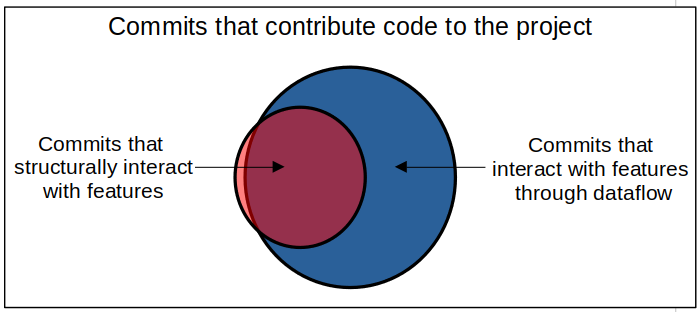
\includegraphics[height=6cm]{gfx/Commits-of-a-Software-Project.png}
\end{tabular}
\captionof{figure}{Illustration of different commit kinds}
\end{center}
\textsf{
In the first two \textbf{RQs} we have discussed different kinds of commits and the ways in which they interact with features. 
The above figure showcases them in a venn diagram and illustrates the dependencies and divisions between them.
}

\section{Operationalization}\label{sec:operationalization}

Here, we explain how the proposed RQs can be answered.
The general experiment process is the same for all RQs.
At first, we collect data comprimising all structural or dataflow-based CFIs by creating reports of a specific type for a chosen software project.
The collected data is then processed in order to gain information for each commit or feature in the project, such as the number of interacting commits and size of a feature.
The processed data is used to calculate statistical information, such as the mean and variance, or the strength of a correlation.
To facilitate a faster and better understanding of the processed data and calculated statistics, we display them graphically via distribution or regression plots.
The projects we investigate in this work, for example \textsc{xz} and \textsc{gzip}, are of a small size and are used in a compression domain.
This choice is based on the fact, that our research intends to only lay basic groundwork, where smaller projects can already offer a lot of insight.
Since we only investigate a few projects, we chose them to be of a similar domain, such that a comparison between them makes more sense.
In the following sections, we explain our method of investigation in more detail for each RQ.

\subsection*{\textbf{RQ1: How do commits and features structurally interact with each other?}}

For this RQ, we examine the interactions contained in the structural reports created with our implementation in VaRA.

\subsubsection*{Patterns around Feature Development}

As there could be vast differences between the projects, we also work with and present their respective data separately.
From the collected structural reports, we first extract the number of structurally interacting commits and size for each feature.
For each interacting commit, we also determine the nesting degree of its structural interaction with the feature.
Additionally to the normal size of a feature, which we call \textsf{potential} size here, we calculate its \textsf{definite} size as well. 
The datapoints of the two properties are shown in two respective bar plots, where the values for each feature are shown in a separate bar.
The bars are labelled after the name of the feature they present, to allow for comparisons between the two plots and between different projects.
For comparisons between the investigated projects, we also calculate the average number of interacting commits and size for each project.
In the plot displaying the number of interacting commits, we stack the commits according to the nesting degree of their respective interaction with the feature.
The first part of each bar consists of commits interacting at a nesting degree of one, the second part of commits interacting at a higher nesting degree.
We do the same in the second plot, where the definite size forms the base of each bar upon which the difference with the potential size is added.
Finally, we relate the two investigated properties in a regression plot.

\subsubsection*{Usage of Commits in Feature Development}

From the commits structurally interacting with features, we calculate the average number of features that a commit changes.
Using the calculated average, we can determine if commits are primarily used to change just one feature.
Additionally, we determine what fraction of commits that structurally interact with features do so with more than one feature, allowing us to see how likely commits are to affect code of only a single or more features.
Here, filtering outliers can help produce more sensible data, as commits responsible for refactoring could change many features, while not implementing any functionality. 






















\subsection*{\textbf{RQ2: How do commits interact with features through dataflow?}}
an initial step of evaluating what fraction of commits affect features through dataflow, is first determining which set of commits we consider in our analysis \\
- logically, we should only consider commits that could potentially be part of a dataflow-based CFI \\
- the only prerequesite is for commits is to be represented by commit regions inside a program \\
The projects investigated for dataflow-based CFIs are the same projects as investigated for structural CFIs.
This choice gives us more insight into a single project and allows us to combine both analysis results as will be discussed below.
For this RQ, we consider all commits that currently contribute code to the repository, 
which we can extract from high level repository information of the project.
We process the collected data, such that, for each commit, we save how many features they interact with through dataflow.
Here, we also indicate whether a commit structurally interacts with a feature, which we can simply check by examining the according structural report.
With this information, we are able to separate commits into ones that implement parts of a feature and those that do not. 
We have already dicussed that commits used to implement a feature are much more likely to account for dataflow interactions.
We provide evidence for this by comparing the average amount of features the two types of commits affect through dataflow. 
Besides that we compute what fraction of commits have dataflow-based interactions with other features, once for all commits, once for commits that are part of a feature and once for commits that aren't part of a feature.
This shows how often commits affect features through dataflow based on their intended purpose, e.g. actively changing the functionality of a feature or changing something seemingly unrelated to a feature. 
With the data collected for each commit, we also plot the distribution of how many features they interact with.
This lets us recognize potential outliers, for example commits with much more dataflow interactions than the mean would suggest.
To check whether feature size is the driving factor in the number of outside commits affecting a feature through dataflow, we compute how strongly the two are correlated.
While we already know the size of each feature from RQ1, it's still neccesary to calculate, for each feature, which commits have dataflow-based interaction with them and subsequently filtering the commits that are part of a feature.

\subsection*{\textbf{RQ3: How do authors interact with features?}}

Here, we also examine the same projects as in the previous RQs.
That way we can reuse data produced in RQ1 to map each feature to the authors that implemented it.
For RQ1 we have already mapped each feature to the commits it interacts with, i.e. that contribute code to it.
It's possible to extract the authors of these commits by accessing high-level repository information.
This directly gives us the authors that implemented a feature.
With the processed data, we are able to calculate the average number of authors used to implement a feature and plot their distribution for a sound overview.
The size of each feature has also been calculated to answer the previous RQs.
With this information we aim to correlate the size of a feature with the amount of authors that implemented it in a regression analysis.
